\documentclass[a4paper, 11pt]{article}

%Comandos para configurar el idioma
\usepackage[spanish,activeacute]{babel}
\usepackage[utf8]{inputenc}
\usepackage[T1]{fontenc} %Necesario para el uso de las comillas latinas.

%Importante que esta sea la última órden del preámbulo
\usepackage{hyperref}
\hypersetup{
  pdftitle={Mecánica Celeste - Simulación del Sistema Solar},
  pdfauthor={Alejandro García Montoro,
          Ana Isabel Ruiz Arroyo,
          Manuel Ruiz Cárdenas,
          Antonio Solís Izquierdo},
  unicode,
  plainpages=false,
  colorlinks,
  citecolor=black,
  filecolor=black,
  linkcolor=black,
  urlcolor=black,
}

\newcommand\fnurl[2]{%
  \href{#2}{#1}\footnote{\url{#2}}%
}

%Paquetes matemáticos
\usepackage{amsmath,amsfonts,amsthm}
\usepackage{enumerate} %Personalización de enumeraciones
\usepackage{tikz} %Dibujos

%Tipografía escalable
\usepackage{lmodern}
%Legibilidad
\usepackage{microtype}

%Código
\usepackage{listings}
\usepackage{color}

\definecolor{dkgreen}{rgb}{0,0.6,0}
\definecolor{gray}{rgb}{0.5,0.5,0.5}
\definecolor{mauve}{rgb}{0.58,0,0.82}

\lstset{frame=tb,
  language=python,
  aboveskip=3mm,
  belowskip=3mm,
  showstringspaces=false,
  columns=flexible,
  basicstyle={\small\ttfamily},
  numbers=left,
  numberstyle=\tiny\color{gray},
  keywordstyle=\color{blue},
  commentstyle=\color{gray},
  stringstyle=\color{mauve},
  breaklines=true,
  breakatwhitespace=true,
  tabsize=3
}

\title{Mecánica Celeste \\ Simulación del Sistema Solar}
\author{Alejandro García Montoro\\
        Ana Isabel MC\\
        Manuel Ruiz Cárdenas\\
        Antonio Solís Izquierdo}
\date{\today}

\begin{document}

  \maketitle

  \section{Introducción}
  Este documento describe la simulación del Sistema Solar implementada por los autores. En la primera sección se explica el proceso de instalación para usuarios de GNU/Linux; en la segunda, se da una breve descripción de los controles disponibles; en la tercera, se describe con detalle el trabajo matemático y su implementación.

  Una versión actualizada de esta documentación, así como del código del programa, puede encontrarse en \fnurl{el repositorio de GitHub kepler\_laws}{https://github.com/agarciamontoro/kepler_laws}.

  \section{Descarga e instalación}
  \subsection{Dependencias}
  Para la correcta ejecución del programa, el sistema sobre el que se instale necesita tener las siguientes dependencias:

  \begin{itemize}
      \item OpenGL (con freeGLUT)
      \item SciPy
      \item wxPython
  \end{itemize}

  La mayoría de las distribuciones de Linux tienen estos paquetes en sus repositorios oficiales.

  En \textbf{Ubuntu}, por ejemplo, la siguiente orden es suficiente para instalar todo lo necesario:

  \begin{lstlisting}
      sudo apt-get install python-opengl freeglut3 python-scipy python-wxgtk2.8
  \end{lstlisting}

  En \textbf{Arch Linux} es muy parecido:

  \begin{lstlisting}
      pacaur -S python-opengl freeglut python-scipy wxpython
  \end{lstlisting}

  \subsection{Descarga del programa}
  Si aún no los tienes, usa el siguiente enlace para descargar todos los ficheros del programa ---incluida esta documentación--- en tu ordenador:

  \fnurl{kepler\_laws-master.zip}{https://github.com/agarciamontoro/kepler\_laws/archive/master.zip}

  Una vez descargado, descomprímelo y abre una terminal en la carpeta donde se encuentren todos los archivos.

  \section{Uso}

  Para comenzar el programa, basta con ejecutar la siguiente orden desde la terminal:

  \begin{lstlisting}
      python2 main.py
  \end{lstlisting}

  \subsection{Controles}

  Se puede rotar la escena haciendo click con el ratón en cualquier lugar de la imagen y moviéndolo. Además, se puede controlar el zoom con la rueda.

  Para controlar la velocidad de la animación -que por defecto se comporta de manera que por cada segundo de la vida real transcurra un día en la simulación- se usan las siguientes teclas:

  \begin{enumerate}
      \item \textbf{X}: Acelera un paso la animación; es decir, añade un día de la simulación por cada segundo de la vida real.
      \item \textbf{Z}: Decelera un paso la animación. Se puede usar repetidamente esta tecla para revertir el tiempo.
  \end{enumerate}

  Para terminar el programa, pulsar la tecla \textbf{Q} o cerrar la ventana de la simulación.

  La interfaz gráfica que se muestra junto a la ventana de la animación permite:

  \begin{enumerate}
      \item Seleccionar los planetas cuya órbita se desea visualizar.
      \item Trasladar la fecha de la animación a un día concreto y mostrar la información relevante de cada planeta marcado.
      \item Introducir un ángulo en radianes, seleccionar un planeta, y calcular la fecha en la que su anomalía excéntrica coincide con el ángulo introducido.
  \end{enumerate}

  \section{Descripción del trabajo}
  \subsection{Unión de trabajos individuales}
  Este trabajo se ha construido sobre las implementaciones que los integrantes del grupo habían desarrollado individualmente.

  Así, al principio ya disponíamos de:
  \begin{enumerate}
      \item Cálculo de las posiciones $x(t)$ de todos los planetas dado un tiempo $t$, basado en el cálculo de la anomalía excéntrica con el algoritmo de Newton-Raphson.
      \item Cálculo de la energía y del momento angular. Estas funciones se han calculado directamente a partir de las definiciones; es decir:
      \begin{align*}
          E(t) &= \frac{1}{2}\lVert\dot{x}\rVert^2 + \frac{\mu}{\lVert x\rVert} \\
          c &= x \wedge \dot{x}
      \end{align*}
      Así, al resultar constantes ambos valores, se ha observado que la implementación es correcta.
  \end{enumerate}

  \subsection{Mejoras matemáticas}

  A partir de este trabajo individual, los integrantes del grupo hemos implementado las siguientes mejoras en la parte matemática del programa:

  \begin{enumerate}
      \item Se ha aplicado la rotación real de los planos de las órbitas con respecto al plano de la eclíptica. Esta rotación se ha calculado obteniendo la matriz de giro a partir del ángulo de inclinación, del ángulo con respecto a la línea de nodos y del ángulo con respecto al eje de excentricidad.
      \item Se ha añadido el cálculo de la fecha en la que un planeta tiene una anomalía excéntrica dada.
  \end{enumerate}

  \subsubsection{Rotación de los planos orbitales}

  La implementación del código de rotación de los planos de las órbitas es el siguiente:

  \begin{lstlisting}
  def getGUICoords(self, pos):
      """Coordinates translation and plane rotation. For visual purposes only.

      Translates 2D coordinates in a XY plane to 3D coordinates in a
      XYZ OpenGL space -i.e., X horizontal axis; Y vertical axis; Z 'depth'
      axis, with Z decreasing from the monitor towards the user-.
      Furthermore, it rotates the orbit plane with the matrix rotation
      of the tilt angle, the node line angle and the eccentricity angle.

      Args:
          pos: 2D coordinates in a [x,y] form

      Returns:
          The pos coordinates translated to the 3D OpenGL world, after have
          applied the rotation of the orbit planes with respect to the
          ecliptic plane.
      """

      i = self.tilt_angle
      big_o = self.node_angle
      small_o = self.ecc_angle

      cos = math.cos
      sin = math.sin

      # Rotation matrix
      m_11 = -cos(big_o)*cos(small_o)*cos(i) + sin(big_o)*sin(small_o)
      m_12 = -cos(i)*sin(small_o)*cos(big_o) - sin(big_o)*cos(small_o)
      m_13 = cos(big_o)*sin(i)

      m_21 = -cos(i)*cos(small_o)*sin(big_o) - cos(big_o)*sin(small_o)
      m_22 = -sin(big_o)*cos(i)*sin(small_o) + cos(big_o)*cos(small_o)
      m_23 = sin(big_o)*sin(i)

      m_31 = sin(i)*cos(small_o)
      m_32 = sin(i)*sin(small_o)
      m_33 = cos(i)

      matrix = [
          [m_11, m_12, m_13],
          [m_21, m_22, m_23],
          [m_31, m_32, m_33]
      ]

      GUI_coords = []

      pos.append(0.0)

      # Matrix product (apply rotation)
      for row, coord in zip(matrix, pos):
          GUI_coords.append(scalarProduct(row, pos))

      # XYZ coordinates are translated into OpenGL as XZ-Y coordinates
      return [GUI_coords[0], GUI_coords[2], -GUI_coords[1]]
  \end{lstlisting}

  En la figura \ref{fig_ani} se puede observar cómo las órbitas no son ya coplanarias como lo eran antes, ni tienen el eje de excentricidad apoyado en el eje de coordenadas $X$.

  \begin{figure}[ht!]
      \centering
      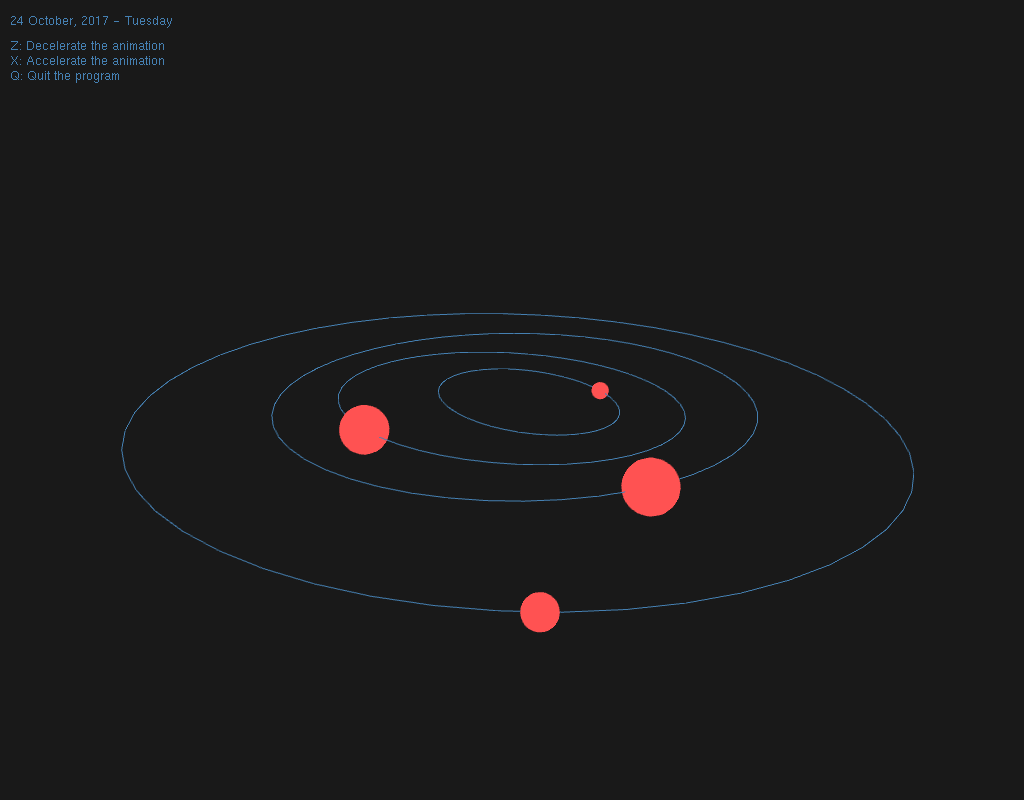
\includegraphics[width=140mm]{./screenshot_ANI.png}
      \caption{Rotación de los planos orbitales con respecto al plano de la eclíptica.\label{fig_ani}}
  \end{figure}

  \subsubsection{Cálculo de la fecha dada la anomalía excéntrica}

  El código que implementa el cálculo de la fecha dada una anomalía excéntrica es el siguiente:

  \begin{lstlisting}
  def getDate(self, u):
      """Retrieves the date from the eccentric anomaly

      Obtains the date in which the eccentric anomaly of the planet is the
      given one.

      Args:
          u: Eccentric anomaly, in radians.

      Returns:
          The (first after self.t0) date -codified as a datetime object- in
          which the planet had the given u.
      """
      p = self.period
      e = self.eccentricity

      delta = p * (u - e*math.sin(u)) / (2*math.pi)

      return self.t0 + timedelta(days=delta)
  \end{lstlisting}

  \subsection{Mejoras gráficas}

  Además del trabajo matemático, se ha mejorado notablemente la interacción gráfica con el programa. Se ha implementado una interfaz que permite al usuario acceder a la información relevante de todos los planetas en fechas arbitrarias mientras se simula el movimiento gráficamente. La figura \ref{fig_gui} muestra la interfaz diseñada.

    \begin{figure}[ht!]
        \centering
        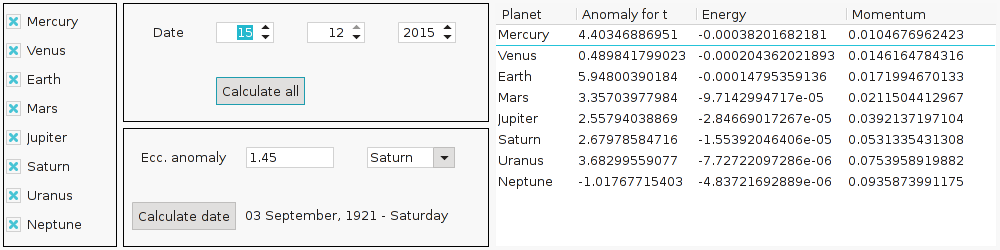
\includegraphics[width=140mm]{./screenshot_GUI.png}
        \caption{Captura de pantalla de la interfaz gráfica implementada. \label{fig_gui}}
    \end{figure}

\end{document}
